\section{Durchführung}
\label{sec:Durchführung}
\subsection{Vorbereitungsaufgaben}
\label{sec:vorbereitung}
In folgender Tabelle sind die recherchierten Werte für die Energien der Kupfer $K_{alpha}$ und $K_{beta}$
Linien zusammengefasst.
\begin{table}[H]
    \centering
    \caption{Literaturwerte der Energien der Spektrallinien von Kupfer. \cite{AP03}.}
    \label{tab:Literaturwerte}
    \sisetup{table-format=1.8}
    \begin{tabular}{S S}
      \toprule
      {Spektrallinie} & {Energie [\si{\kilo\electronvolt}]} \\
      \midrule
    {$K_{\alpha}$} & 8.048 \\
    {$K_{\beta} $} & 8.907 \\
      \bottomrule
    \end{tabular}
  \end{table}
\noindent

\subsection{Der Versuchsaufbau}
Für die Erzeugung der benötigten Röntgenstrahlung wird eine Kupfer-Röntgenröhre verwendet. Die Röntgenstrahlung wird aus dieser auf den LiF-Kristall oder den Plexiglasstreuer geschossen. Der Winkel des
LiF-Kristalls oder Plexiglasstreuers kann verstellt werden. Hinter dem LiF-Kristall/Plexiglasstreuers befindet sich ein Geiger-Müller-Zählrohr, welches ebenfalls auf unterschiedliche Winkel einstellbar ist.
Dies ist in Abbildung \ref{fig:versuchsaufbau1} dargestellt.
\begin{figure}[H]
  \centering
  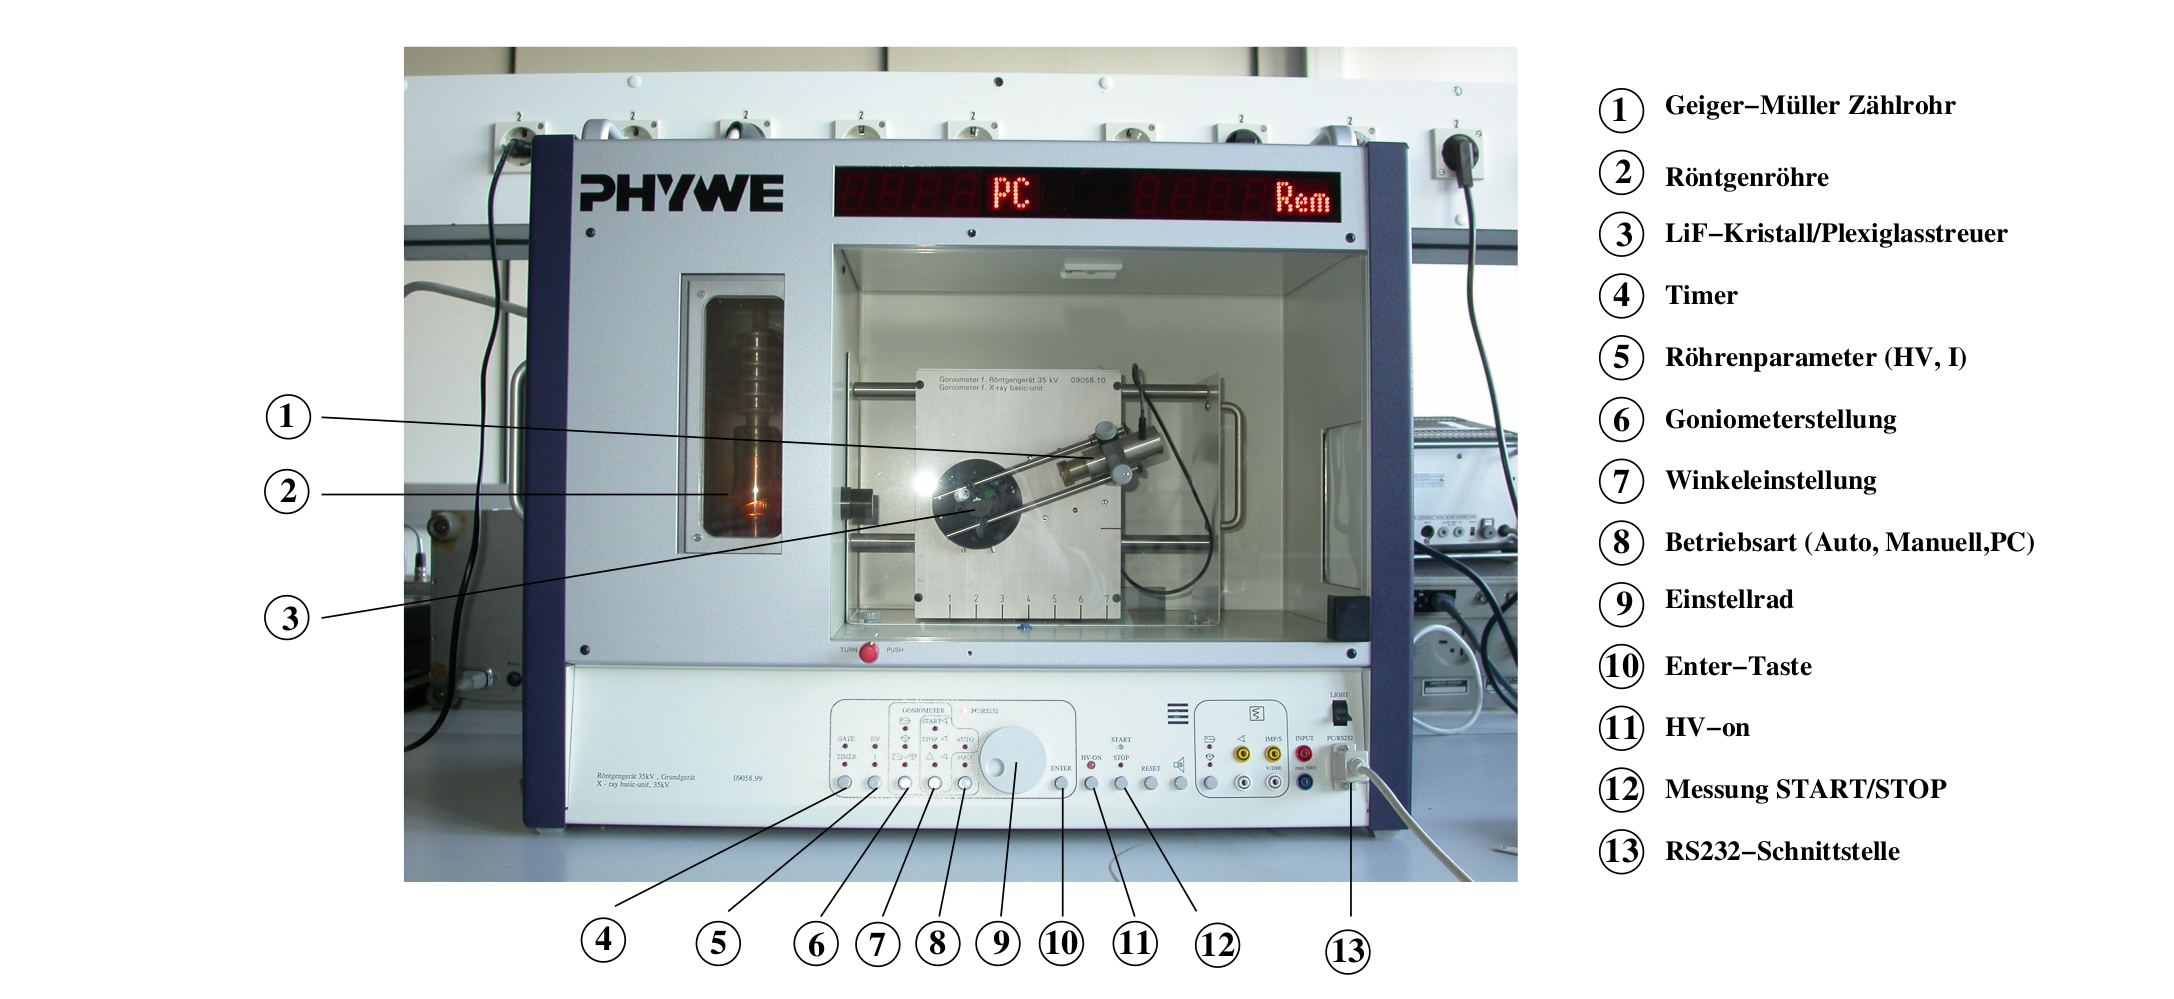
\includegraphics[scale=0.23]{content/versuchsaufbau1.png}
  \caption{Der Versuchsaufbau. \cite{AP01}}
  \label{fig:versuchsaufbau1}
\end{figure}

\subsection{Durchführung des Versuches}
Zu Beginn wird das Emissionspektrum bei einer Blendenbreite von $2 \si{\milli\meter}$ und dem LiF-Kristall gemessen. Dabei wird in $0.1 \si{\degree}$-Schritten bei der Beugungsordnung $n = 1$ eine Messung des
Röntgenspektrums vorgenommen. Dann wird die Intensität an einem Aluminium-Absorber gemessen. Dabei wird eine $2 \si{\milli\meter}$ -Blende verwendet. Es wird auch eine Messung ohne Aluminium-Absorber
durchgeführt.
Um bei der Messung die Totzeit des Geiger-Müller-Zählrohres zu beachten, muss folgende Korrektur vorgenommen werden:
\begin{equation}
	I = \frac{N}{1 - \tau \cdot N}.
  \label{eqn:(4)}
\end{equation}
Hierbei bezeichnet $\tau = 90 \mu \si{\second}$ die Totzeit des Geiger-Müller-Zählrohres und $N$ die Anzahl der Photonen.
Die gemessenen Spektren $I_{Al}$ und $I_0$ ergeben nach
\begin{equation}
	T(\lambda) = \frac{I_{Al}}{I_0}
	\label{eqn:trans}
\end{equation}
die Transmission an dem LiF-Kristall in Abhängigkeit der Wellenlänge.
Es wird eine zweite Messung durchgeführt, wobei der LiF-Kristall durch den Plexiglas-Absorber und die $2 \si{\milli\meter}$-Blende gegen eine $\SI{5}{\milli\meter}$-Blende getauscht wird.
Um die Intensität der Cu-Röhre zu bestimmen, wird nun der Plexiglasstreuer auf $\SI{45}{\degree}$ und das Geiger-Müller-Zählrohr auf $\SI{90}{\degree}$ eingestellt. Dann wird die Intensität der Cu-Röhre gemessen.
Für die Bestimmung der Compton-Wellenlänge wird zuerst die Intensität bei nicht gestreuter Röntgenstrahlung mit Aluminiumabsorber im Strahlengang zwischen Röntgenröhre und Streukörper,
dann die Intensität bei gestreuter Röntgenstrahlung mit Aluminiumabsorber im Strahlengang zwischen Streukörper und Geiger-Müller-Zählrohr gemessen.
Dies ist in Abbildung \ref{fig:versuchsaufbau2} dargestellt.

\begin{figure}[H]
  \centering
  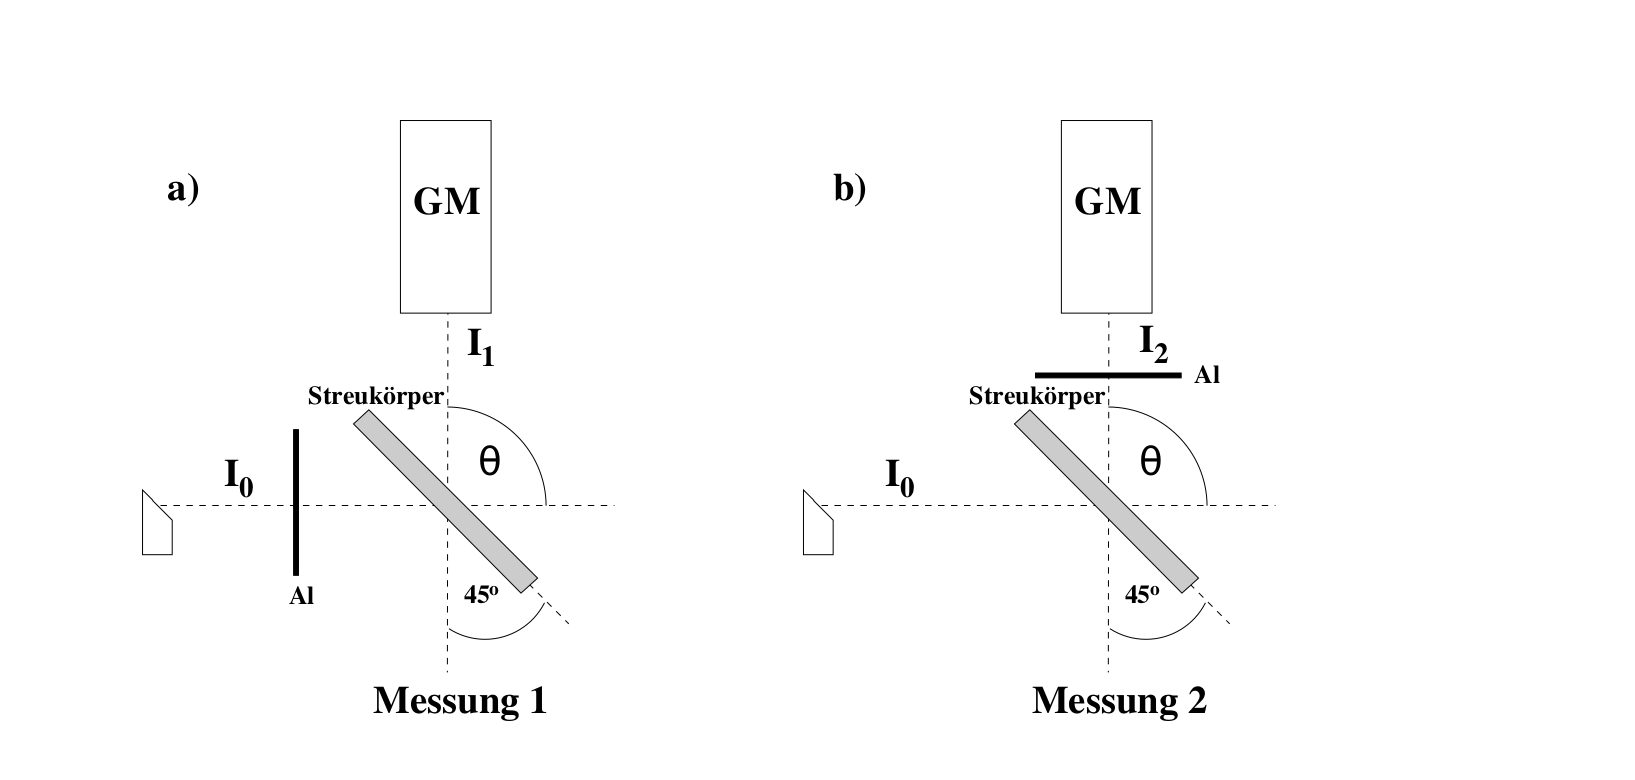
\includegraphics[scale=0.3]{content/versuchsaufbau2.png}
  \caption{Der Versuchsaufbau bei der Transmissionsbestimmung. \cite{AP01}}
  \label{fig:versuchsaufbau2}
\end{figure}
Die Transmission wird nun nach \eqref{eqn:trans} berechnet.
